\begin{recipe}
    [% 
        preparationtime = {\unit[15]{min}},
        portion = {\portion{4}},
        bakingtime = {\unit[25]{min}}
    ]
    {Aquafaba brownie}
    \introduction{%
        Aquafaba is the viscous water from chickpea can.
        Why should you be bothered?
        You could possibly exchange it for beaten egg whites but I always struggle what to do with leftover yolks.
        Aquafaba is a by-product and it's ingenious it can be turned into desserts.
        Eat chickpea for lunch and aquafaba for afternoon tea - two birds with one stone!
    }

    \ingredients{%
        \unit[200]{g} & Chocolate \\
        \unit[150]{g} & Butter \\
        1 can & Aquafaba \\
        0.75 c. & Sugar \\
        1.25 c. & Flour \\
        Pinch & Salt \\
        \nicefrac{1}{4} ts. & Baking powder \\
        & Chili or cinnamon or vanilla \\
        & Raspberries \\
        & Hazelnuts
    }

    \preparation{%
        \step In a small pot heat up gently butter, chocolate and spices till chocolate melts.

        \step Beat aquafaba in an exactly same way as you would do egg whites.
        At the end add sugar in small portions.
        Gently mix with melted chocolate.

        \step In a separate bowl, mix flour and baking powder.

        \step Gently, in portions, add flour to liquid and stir with a spatula.

        \step Pour cake batter to a baking tin (small, something like 20x25) lined with parchment.
        Decorate with nuts, raspberries and pieces of chocolate.

        \step Bake at \unit[180]{\textcelcius} for 20 min.
        Do not overbake!
    }

    \hint{%
        Add \nicefrac{1}{4} cup of coffee to the first step for extra deep flavour.
    }

\end{recipe}

\begin{figure}[h]
    \centering
    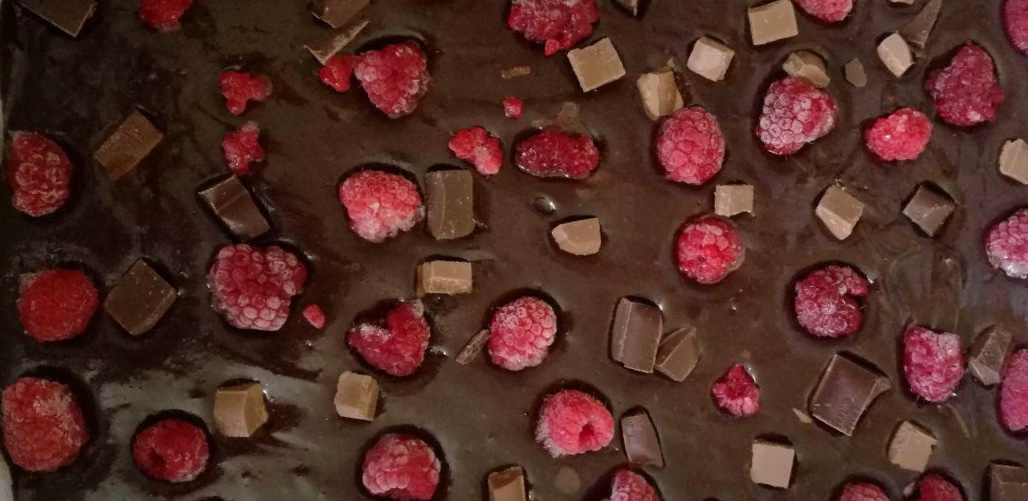
\includegraphics[width=8cm]{pic/brownie}
\end{figure}
